\section{Empirical Evaluation}
\label{sec:exps}

\iftoggle{arxiv}{
In \cref{sec:exp:synthetic} we test Mamba's ability to solve the two synthetic tasks motivated in \cref{sec:method:motivation}.
We then evaluate on three domains, each evaluated on autoregressive pretraining as well as downstream tasks.
\begin{itemize}[leftmargin=*,itemsep=0pt,topsep=0pt]
  \item \cref{sec:exp:language}: language model pretraining (scaling laws), and zero-shot downstream evaluation.
  \item \cref{sec:exp:genomics}: DNA sequence pretraining, and fine-tuning on a long-sequence classification task.
  \item \cref{sec:exp:audio}: audio waveform pretraining, and the quality of autoregressively generated speech clips.
\end{itemize}
Finally, \cref{sec:exp:benchmark} shows Mamba's computational efficiency at both training and inference time,
and \cref{sec:exp:ablations} ablates various components of the architecture and selective SSMs.
}{
  Mamba achieves state-of-the-art results on the synthetic tasks (\cref{sec:exp:synthetic}) and three different domains (language, DNA, audio) (\cref{sec:exp:language,sec:exp:genomics,sec:exp:audio}) on both pretraining and downstream tasks,
  while being very computationally efficient (\cref{sec:exp:benchmark}).
}

\subsection{Synthetic Tasks}
\label{sec:exp:synthetic}

\iftoggle{arxiv}{
  Full experiment details for these tasks including task details and training protocol are in \cref{sec:exp-details:synthetics}.

\subsubsection{Selective Copying}


The Copying task is one of the most well-studied synthetic tasks for sequence modeling,
originally designed to test the memorization abilities of recurrent models.
As discussed in \cref{sec:method:motivation}, LTI SSMs (linear recurrences and global convolutions)
can easily solve this task by only keeping track of time instead of reasoning about the data;
for example, by constructing a convolution kernel of exactly the right length (\cref{fig:copying}).
This was explicitly validated in earlier work on global convolutions~\citep{romero2021ckconv}.
The Selective Copying task prevents this shortcut by randomizing the spacing between tokens.
Note that this task has been introduced before as the Denoising task~\citep{jing2019gated}.

Note that many previous works argue that adding architecture gating (multiplicative interactions) can endow models with ``data-dependence'' and solve related tasks \citep{dao2023hungry,poli2023hyena}.
However, we find this explanation insufficient intuitively because such gating does not interact along the sequence axis, and cannot affect the spacing between tokens.
In particular architecture gating is not an instance of a selection mechanism (\cref{sec:discussion:selection}).

\cref{tab:copying} confirms that gated architectures such as H3 and Mamba only partially improve performance,
while the selection mechanism (modifying S4 to S6) easily solves this task, particularly when combined with these more powerful architectures.



\subsubsection{Induction Heads}

Induction heads~\citep{olsson2022context} is a simple task from the mechanistic interpretability lens~\citep{elhage2021mathematical} that is surprisingly predictive of the in-context learning ability of LLMs. It requires models to perform associative recall and copy: for example, if the model has seen a bigram such as ``Harry Potter'' in the sequence, then the next time ``Harry'' appears in the same sequence, the model should be able to predict ``Potter'' by copying from history.

\paragraph{Dataset.}
We train a 2-layer model on the induction heads task at sequence length $256$, with a vocab size of $16$,
which is comparable to prior work on this task \citep{dao2023hungry} but with longer sequences.
We additionally investigate generalization and extrapolation abilities by evaluating on a range of sequence lengths from $2^6 = 64$ up to $2^{20} = 1048576$ at test time.

\paragraph{Models.}
Following established work on induction heads, we use 2 layer models, which allows attention to mechanistically solve the induction heads task~\citep{olsson2022context}.
We test both multi-head attention (8 heads, with various positional encodings) and SSM variants.
We use a model dimension $D$ of $64$ for Mamba and $128$ for the other models.

\paragraph{Results.}

\cref{fig:induction} shows that
Mamba---or more precisely, its selective SSM layer---has the ability to solve the task perfectly because of its ability to selectively remember the relevant token while ignoring everything else in between.
\textbf{It generalizes perfectly to million-length sequences, or $4000\times$ longer than it saw during training},
while no other method goes beyond $2\times$.

Out of positional encoding variants for attention models, xPos (which was designed for length extrapolation) is slightly better than the others;
also note that all attention models were only tested up to sequence length $2^{14}=16384$ due to memory limitations.
Out of other SSMs, H3 and Hyena are similar, contrary to the findings in \citet{poli2023hyena}.

%





}{
\cref{tab:copying} and \cref{fig:induction} show results for the synthetic tasks.
On Selective Copying, the selective SSM layer is enough to solve the task independently of the architecture used,
while previous LTI SSMs cannot even when combined with more powerful architectures.
On Induction Heads, Mamba learns the task perfectly and can even extrapolate to
million-length sequences, or $4000\times$ longer than it saw during training,
while no other method goes beyond $2\times$.
Full discussion for synthetic tasks are in \cref{sec:exp-full:synthetic}.
}


\begin{figure*}
  \begin{minipage}{0.33\linewidth}
    \iftoggle{arxiv}{\small}{\footnotesize}
    \centering
    \begin{tabular}{@{}llll@{}}
      \toprule
      \textsc{Model}          & \textsc{Arch.}        & \textsc{Layer}      & \textsc{Acc.} \\
      \midrule
      S4                       & No gate               & S4                  & 18.3 \\
      -                       & No gate               & S6                  & \textbf{97.0} \\
      \midrule
      H3                      & H3                    & S4                  & 57.0 \\
      Hyena                   & H3                    & Hyena               & 30.1 \\
      -                       & H3                    & S6                  & \textbf{99.7} \\
      \midrule
      -                       & Mamba                 & S4                  & 56.4 \\
      -                       & Mamba                 & Hyena               & 28.4 \\
      Mamba                   & Mamba                 & S6                  & \textbf{99.8} \\
      \bottomrule
    \end{tabular}
    \iftoggle{arxiv}{
      \captionsetup{type=table,skip=12pt}
    }{
      \captionsetup{type=table,skip=12pt}
    }
    \caption{
      (\textbf{Selective Copying}.) \\
      Accuracy for combinations of architectures and inner sequence layers.
    }
    \label{tab:copying}
  \end{minipage}
  \hfill
  \begin{minipage}{\iftoggle{arxiv}{0.55\linewidth}{0.63\linewidth}}
    \centering
    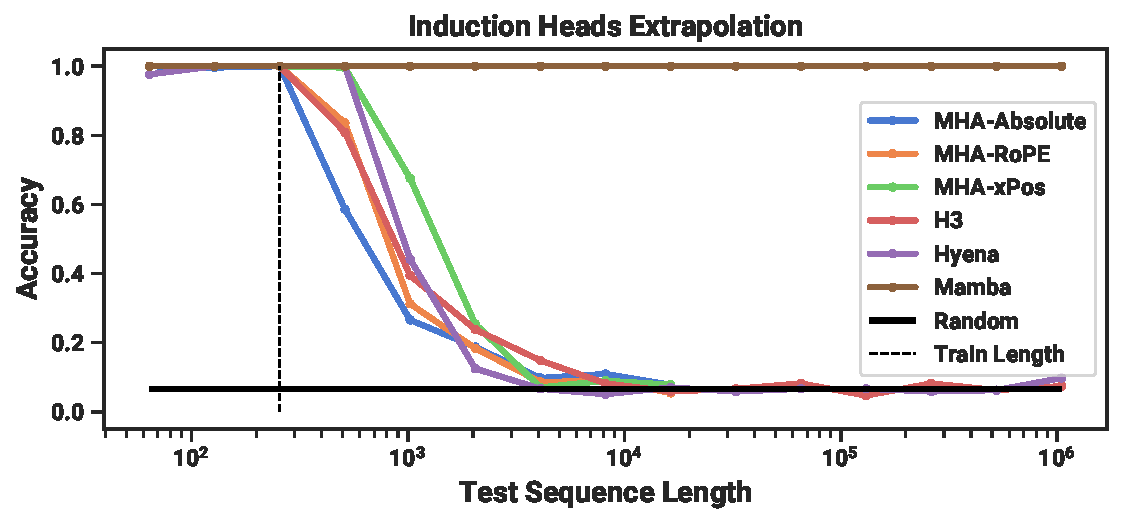
\includegraphics[width=\linewidth]{fig/induction.pdf}
    \iftoggle{arxiv}{
      \captionsetup{type=table,skip=-6pt}
    }{
      \captionsetup{type=figure,skip=-12pt}
    }
    \caption{
      (\textbf{Induction Heads}.)
      Models are trained on sequence length $2^8=256$, and tested on increasing sequence lengths of $2^6=64$ up to $2^{20}=1048576$.
      Full numbers in \cref{tab:induction}.
    }
    \label{fig:induction}
  \end{minipage}
\end{figure*}


\subsection{Language Modeling}
\label{sec:exp:language}

We evaluate the Mamba architecture on standard autoregressive language modeling against other architectures, on both pretraining metrics (perplexity) and zero-shot evaluations.
We set the model sizes (depth and width) to mirror GPT3 specifications. %
We use the Pile dataset~\citep{pile}, and follow the training recipe described in~\citet{brown2020language}. 
All training details are in~\cref{sec:exp-details:lm}.


\iftoggle{arxiv}{
  \subsubsection{Scaling Laws}
}{
  \para{Scaling Laws.}
}
For baselines, we compare against the standard Transformer architecture (GPT3 architecture), as well as the strongest Transformer recipe we know of (here referred to as Transformer++), based on the PaLM and LLaMa architectures (e.g.\ rotary embedding, SwiGLU MLP, \iftoggle{arxiv}{RMSNorm instead of LayerNorm, no linear bias, and higher learning rates}{etc.}).
We also compare against other recent subquadratic architectures (\cref{fig:lm-scaling}).
All model details are in \cref{sec:exp-details:lm}.

\iftoggle{arxiv}{
\cref{fig:lm-scaling} shows scaling laws under the standard Chinchilla~\citep{hoffmann2022empirical} protocol,
on models from $\approx 125M$ to $\approx 1.3B$ parameters.
\textbf{Mamba is the first attention-free model to match the performance of a very strong Transformer recipe (Transformer++) that has now become standard,
particularly as the sequence length grows.}
(We note that full results on context length 8k are missing for the RWKV and RetNet baselines,
prior strong recurrent models that can also be interpreted as SSMs, because of a lack of efficient implementations leading to out-of-memory or unrealistic computation requirements.)
}{}

\begin{figure*}[!t]
  \centering
  \begin{subfigure}[t]{0.49\linewidth}
    \centering
    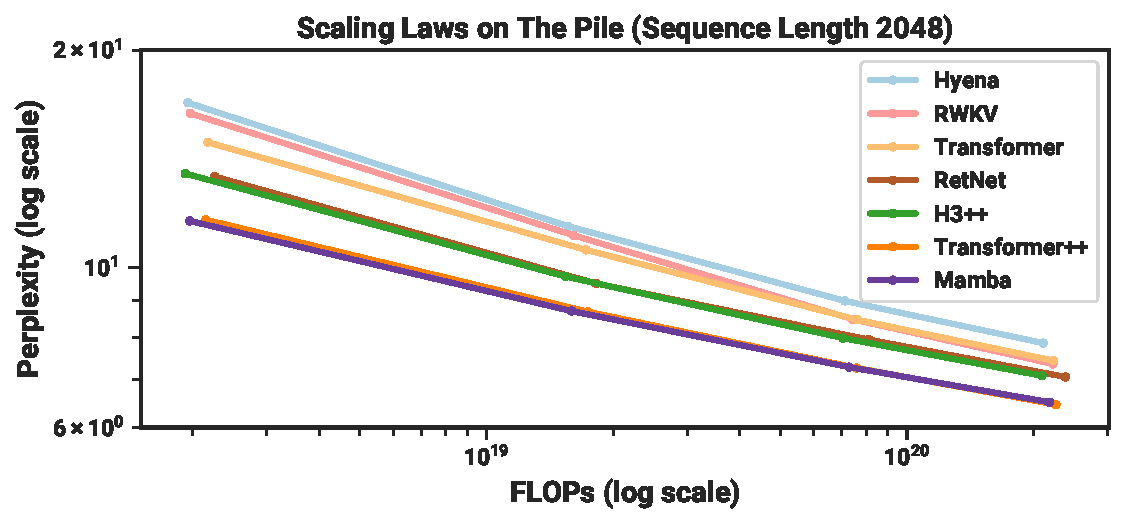
\includegraphics[width=\textwidth]{fig/pile_2k.pdf}
  \end{subfigure}
  \begin{subfigure}[t]{0.49\linewidth}
    \centering
    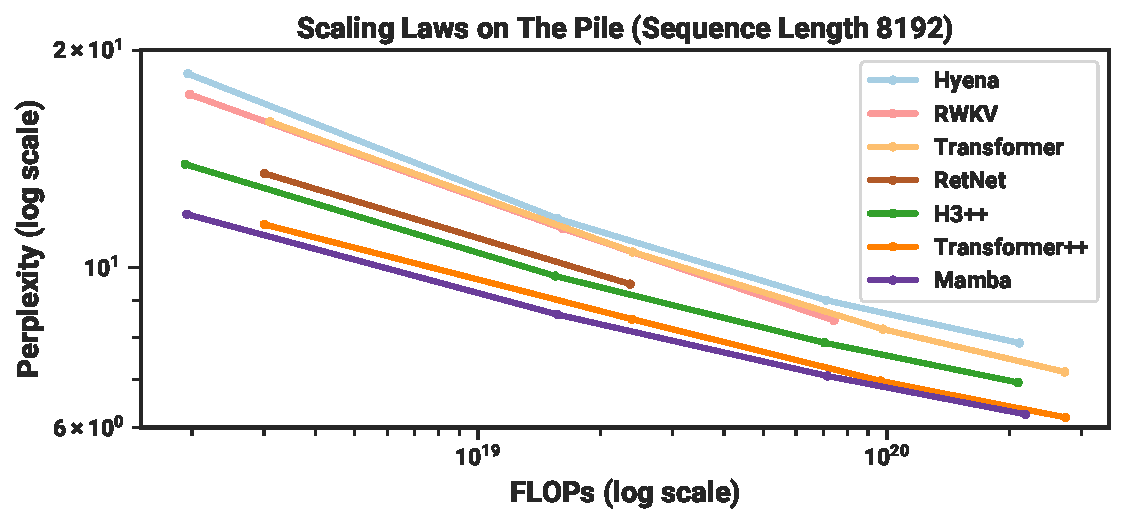
\includegraphics[width=\textwidth]{fig/pile_8k.pdf}
  \end{subfigure}
  \caption{
    (\textbf{Scaling Laws}.) %
    Models of size $\approx 125M$ to $\approx 1.3B$ parameters, trained on the Pile.
    Mamba scales better than all other attention-free models and is the first to match the performance of a very strong ``Transformer++'' recipe that has now become standard,
    particularly as the sequence length grows.
  }
  \label{fig:lm-scaling}
  \iftoggle{arxiv}{}{\vspace{-1em}}
\end{figure*}


\iftoggle{arxiv}{
  \subsubsection{Downstream Evaluations}
}{
  \para{Downstream Evaluations.}
}
\cref{table:downstream_zeroshot} shows the performance of Mamba on a range of popular downstream zero-shot evaluation tasks.
We compare against the most well-known open source models at these sizes,
most importantly Pythia~\citep{biderman2023pythia} and RWKV~\citep{peng2023rwkv} which were trained with the same tokenizer, dataset, and training length (300B tokens) as our models.
\iftoggle{arxiv}{(Note that Mamba and Pythia are trained with context length 2048, while RWKV was trained with context length 1024.)}{}




\begin{table*}[!th]
  \small
  \centering
  \captionsetup{font=small}
  \caption{
    (\textbf{Zero-shot Evaluations}.) Best results for each size in bold.
    We compare against open source LMs with various tokenizers, trained for up to 300B tokens.
    Pile refers to the validation split, comparing only against models trained on the same dataset and tokenizer (GPT-NeoX-20B).
    For each model size, Mamba is best-in-class on every single evaluation result,
    and generally matches baselines at twice the model size.
    %
  }
  \resizebox{0.99\linewidth}{!}
  {
    \begin{tabular}{@{}lllllllllll@{}}
      \toprule
      \sc{Model}                                        & \sc{Token.} & \sc{Pile}             & \sc{LAMBADA}          & \sc{LAMBADA}         & \sc{HellaSwag}       & \sc{PIQA}            & \sc{Arc-E}           & \sc{Arc-C}           & \sc{WinoGrande}      & \sc{Average} \\
                                                        &             & \sc{ppl $\downarrow$} & \sc{ppl $\downarrow$} & \sc{acc $\uparrow$}  & \sc{acc $\uparrow$}  & \sc{acc $\uparrow$}  & \sc{acc $\uparrow$}  & \sc{acc $\uparrow$}  & \sc{acc $\uparrow$}  & \sc{acc $\uparrow$} \\
                                        \midrule
      \iftoggle{arxiv}{
      Hybrid H3-130M                                           & GPT2        & ---                   & 89.48                 & 25.77                & 31.7                 & 64.2                 & 44.4                 & 24.2                 & 50.6                 & 40.1 \\
      Pythia-160M                                       & NeoX        & 29.64                 & 38.10                 & 33.0                 & 30.2                 & 61.4                 & 43.2                 & 24.1                 & \textbf{51.9}        & 40.6 \\
      \textbf{Mamba-130M}                               & NeoX        & \textbf{10.56}        & \textbf{16.07}        & \textbf{44.3}        & \textbf{35.3}        & \textbf{64.5}        & \textbf{48.0}        & \textbf{24.3}        & \textbf{51.9}        & \textbf{44.7} \\
      \midrule
      }{}
      Hybrid H3-360M                                           & GPT2        & ---                   & 12.58                 & 48.0                 & 41.5                 & 68.1                 & 51.4                 & 24.7                 & 54.1                 & 48.0 \\
      Pythia-410M                                       & NeoX        & 9.95                  & 10.84                 & 51.4                 & 40.6                 & 66.9                 & 52.1                 & 24.6                 & 53.8                 & 48.2 \\
      \textbf{Mamba-370M}                               & NeoX        & \textbf{8.28}         & \textbf{8.14}         & \textbf{55.6}        & \textbf{46.5}        & \textbf{69.5}        & \textbf{55.1}        & \textbf{28.0}        & \textbf{55.3}        & \textbf{50.0} \\
      \midrule
      Pythia-1B                                         & NeoX        & 7.82                  & 7.92                  & 56.1                 & 47.2                 & 70.7                 & 57.0                 & 27.1                 & 53.5                 & 51.9 \\
      \textbf{Mamba-790M}                               & NeoX        & \textbf{7.33}         & \textbf{6.02}         & \textbf{62.7}        & \textbf{55.1}        & \textbf{72.1}        & \textbf{61.2}        & \textbf{29.5}        & \textbf{56.1}        & \textbf{57.1} \\
      \midrule
      GPT-Neo 1.3B                                      & GPT2        & ---                   & 7.50                  & 57.2                 & 48.9                 & 71.1                 & 56.2                 & 25.9                 & 54.9                 & 52.4 \\
      Hybrid H3-1.3B                                           & GPT2        & ---                   & 11.25                 & 49.6                 & 52.6                 & 71.3                 & 59.2                 & 28.1                 & 56.9                 & 53.0 \\
      OPT-1.3B                                          & OPT         & ---                   & 6.64                  & 58.0                 & 53.7                 & 72.4                 & 56.7                 & 29.6                 & 59.5                 & 55.0 \\
      Pythia-1.4B                                       & NeoX        & 7.51                  & 6.08                  & 61.7                 & 52.1                 & 71.0                 & 60.5                 & 28.5                 & 57.2                 & 55.2 \\
      RWKV-1.5B                                         & NeoX        & 7.70                  & 7.04                  & 56.4                 & 52.5                 & 72.4                 & 60.5                 & 29.4                 & 54.6                 & 54.3 \\
      \textbf{Mamba-1.4B}                               & NeoX        & \textbf{6.80}         & \textbf{5.04}         & \textbf{64.9}        & \textbf{59.1}        & \textbf{74.2}        & \textbf{65.5}        & \textbf{32.8}        & \textbf{61.5}        & \textbf{59.7} \\
      \midrule
      GPT-Neo 2.7B                                      & GPT2        & ---                   & 5.63                  & 62.2                 & 55.8                 & 72.1                 & 61.1                 & 30.2                 & 57.6                 & 56.5 \\
      Hybrid H3-2.7B                                           & GPT2        & ---                   & 7.92                  & 55.7                 & 59.7                 & 73.3                 & 65.6                 & 32.3                 & 61.4                 & 58.0 \\
      OPT-2.7B                                          & OPT         & ---                   & 5.12                  & 63.6                 & 60.6                 & 74.8                 & 60.8                 & 31.3                 & 61.0                 & 58.7 \\
      Pythia-2.8B                                       & NeoX        & 6.73                  & 5.04                  & 64.7                 & 59.3                 & 74.0                 & 64.1                 & 32.9                 & 59.7                 & 59.1 \\
      RWKV-3B                                           & NeoX        & 7.00                  & 5.24                  & 63.9                 & 59.6                 & 73.7                 & 67.8                 & 33.1                 & 59.6                 & 59.6 \\
      \textbf{Mamba-2.8B}                               & NeoX        & \textbf{6.22}         & \textbf{4.23}         & \textbf{69.2}        & \textbf{66.1}        & \textbf{75.2}        & \textbf{69.7}        & \textbf{36.3}        & \textbf{63.5}        & \textbf{63.3} \\
      \midrule
      GPT-J-6B                                          & GPT2        & --                    & 4.10                  & 68.3                 & 66.3                 & 75.4                 & 67.0                 & 36.6                 & 64.1                 & 63.0 \\
      OPT-6.7B                                          & OPT         & --                    & 4.25                  & 67.7                 & 67.2                 & 76.3                 & 65.6                 & 34.9                 & 65.5                 & 62.9 \\
      Pythia-6.9B                                       & NeoX        & 6.51                  & 4.45                  & 67.1                 & 64.0                 & 75.2                 & 67.3                 & 35.5                 & 61.3                 & 61.7 \\
      RWKV-7.4B                                         & NeoX        & 6.31                  & 4.38                  & 67.2                 & 65.5                 & 76.1                 & 67.8                 & 37.5                 & 61.0                 & 62.5 \\
      \bottomrule
    \end{tabular}
  }
  \label{table:downstream_zeroshot}
\end{table*}

\subsection{DNA Modeling}
\label{sec:exp:genomics}

Motivated by the success of large language models, there
has been recent exploration into using the foundation model paradigm for genomics.
DNA has been likened to language in that it consists of sequences of discrete tokens with a finite vocabulary.
It is also known for requiring long-range dependencies to model \citep{avsec2021effective}.
We investigate Mamba as a FM backbone for pretraining and fine-tuning in the same setting as recent works on long-sequence models for DNA \citep{nguyen2023hyenadna}.
In particular, we focus on two explorations of scaling laws across model size and sequence length (\cref{fig:dna}), and a difficult downstream synthetic classification task requiring long context (\cref{fig:species}).
\iftoggle{arxiv}{

  
For pretraining, we largely follow a standard causal language modeling (next token prediction) setup for the training and model details (see also \cref{sec:exp-details:lm}).
For the dataset, we largely follow the setup of HyenaDNA~\citep{nguyen2023hyenadna}, which uses the HG38 dataset for pretraining consisting of a single human genome
with about 4.5 billion tokens (DNA base pairs) in the training split.

\subsubsection{Scaling: Model Size}


In this experiment, we investigate the scaling properties of genomics foundation models with various model backbones (\cref{fig:dna} \textit{Left}).
%


\para{Training.}
To advantage the baselines, we train on a short sequence length of $1024$; as shown in \cref{sec:exp:dna:length}, we expect results to favor Mamba even more at longer sequence lengths.
We fix a global batch size of $1024$, for a total of $2^{20} \approx 1M$ tokens per batch.
Models were trained for $10K$ gradient steps for a total of $10B$ tokens.

\para{Results.}
\cref{fig:dna} (\emph{Left}) shows that Mamba's pretraining perplexity improves smoothly with model size,
and that Mamba scales better than both HyenaDNA and Transformer++.
For example, at the largest model size of $\approx 40M$ parameters,
the curve shows that \textbf{Mamba can match the Transformer++ and HyenaDNA models with roughly $3\times$ to $4\times$ fewer parameters}.


\subsubsection{Scaling: Context Length}
\label{sec:exp:dna:length}

In the next DNA experiment, we investigate the scaling properties of models with respect to sequence length.
We only compare the HyenaDNA and Mamba models, as quadratic attention becomes prohibitively expensive at longer sequence lengths.
We pretrain models on sequence lengths $2^{10}=1024$, $2^{12}=4096$, $2^{14}=16384$, $2^{16}=65536$, $2^{18}=262144$, $2^{20}=1048576$.
We fix a model size of 6 layers by width $128$ (about 1.3M-1.4M parameters).
Models were trained for $20K$ gradient steps for a total of $\approx 330B$ tokens.
The longer sequence lengths used sequence length warmup similar to \citep{nguyen2023hyenadna}.

\para{Results.}
\cref{fig:dna} (\emph{Right}) shows that \textbf{Mamba is able to make use of longer context even up to extremely long sequences of length 1M}, and its pretraining perplexity improves as the context increases.
On the other hand, the HyenaDNA model gets worse with sequence length.
This is intuitive from the discussion in \cref{sec:method:properties} on properties of the selection mechanism.
In particular, LTI models cannot selectively ignore information;
from a convolutional perspective, a very long convolution kernel is aggregating all information across a long sequence which may be very noisy.
Note that while HyenaDNA claims to improve with longer context, their results do not control for computation time.


\subsubsection{Synthetic Species Classification}

We evaluate models on a downstream task of classifying between 5 different species by randomly sampling a contiguous segment of their DNA.
This task is adapted from HyenaDNA,
which used the species $\{ \texttt{human}, \texttt{lemur}, \texttt{mouse}, \texttt{pig}, \texttt{hippo} \}$.
We modify the task to be significantly more challenging by classifying between the five \emph{great apes} species \\ $\{ \texttt{human}, \texttt{chimpanzee}, \texttt{gorilla}, \texttt{orangutan}, \texttt{bonobo} \}$,
which are known to share 99\% of their DNA.

}{
  Full discussion for these tasks is in \cref{sec:exp-full:genomics}.
}


\begin{figure*}[!t]
  \centering
\begin{subfigure}{.49\linewidth}%
  \centering
  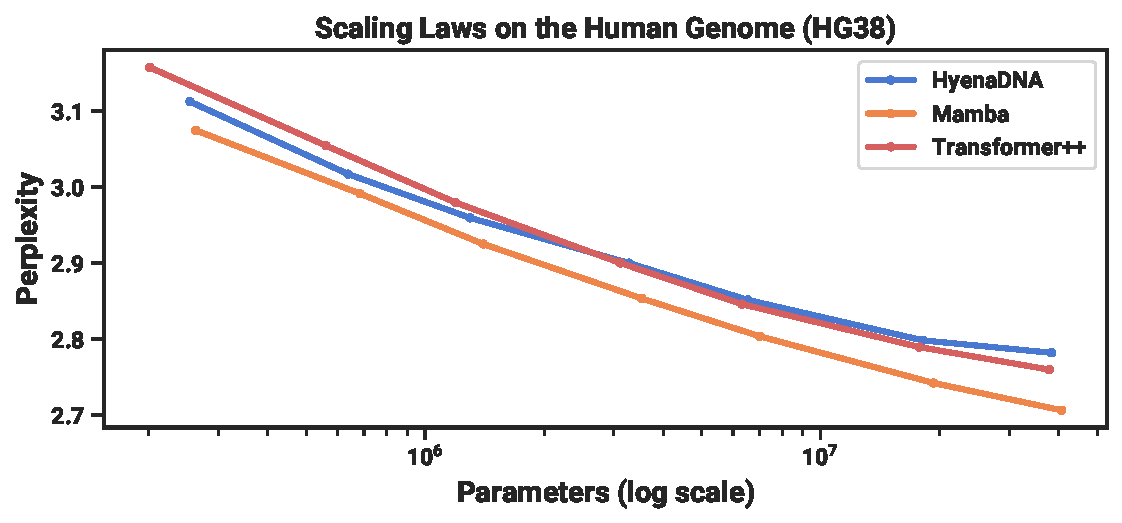
\includegraphics[width=\linewidth]{fig/dna_scaling.pdf}
\end{subfigure}
\begin{subfigure}{.49\linewidth}%
  \centering
  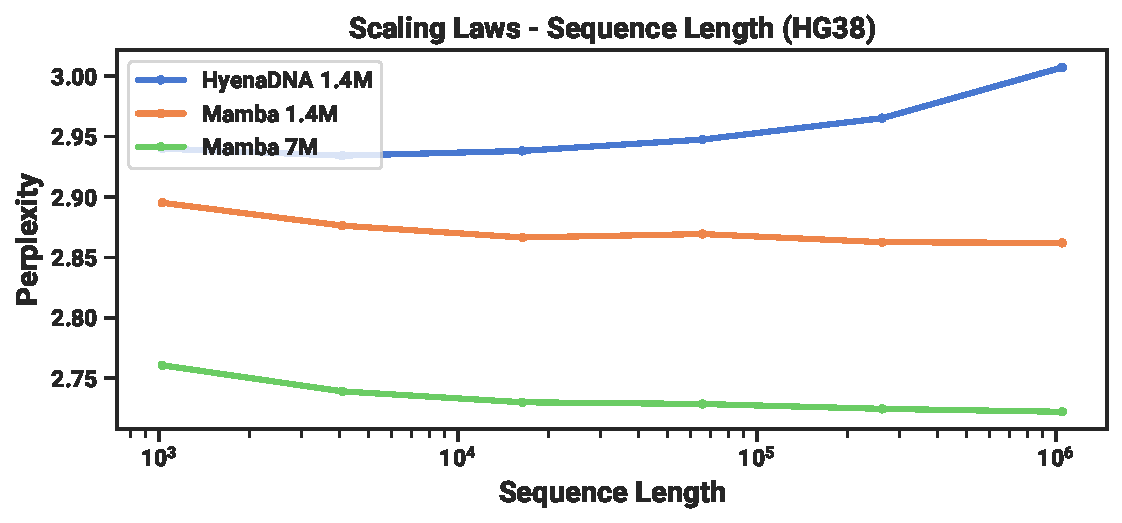
\includegraphics[width=\linewidth]{fig/dna_length.pdf}
\end{subfigure}
\caption{
  (\textbf{DNA Scaling Laws}.) Pretraining on the HG38 (human genome) dataset.
  (\textit{Left}) Fixing short context length $2^{10}=1024$ and increasing size from $\approx200K$ to $\approx 40M$ parameters, Mamba scales better than baselines.
  (\textit{Right}) Fixing model size and increasing sequence lengths while \iftoggle{arxiv}{keeping tokens/batch and total training tokens fixed}{controlling for computation}.
  Unlike baselines, the selection mechanism of Mamba facilitates better performance with increasing context length.
}
\label{fig:dna}
\end{figure*}


\begin{figure*}[!ht]
  \begin{minipage}[t]{.49\linewidth}
    \centering
    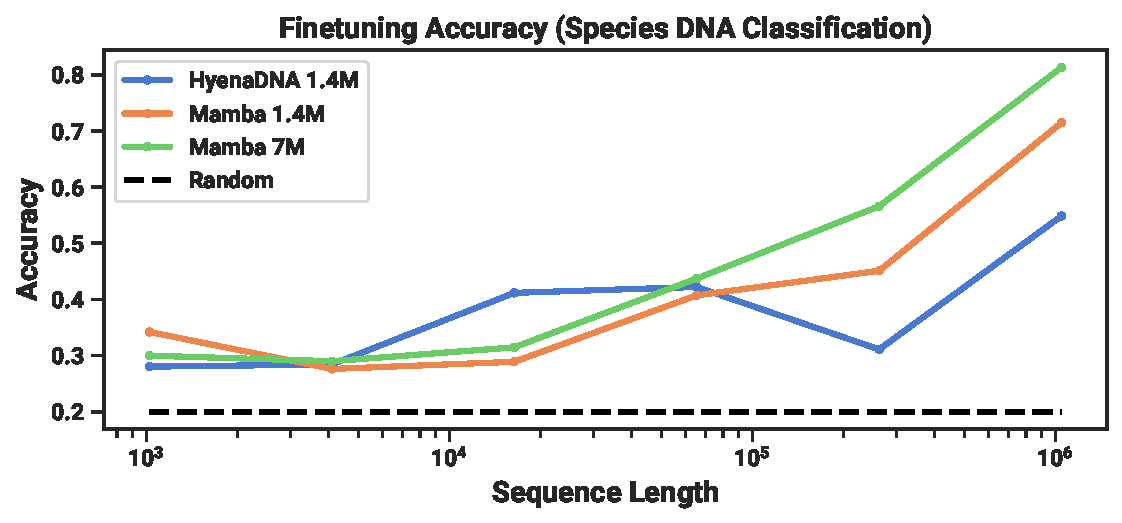
\includegraphics[width=\linewidth]{fig/species.pdf}
    \captionsetup{type=figure}
    \caption{
      (\textbf{Great Apes DNA Classification}.)
      Accuracy after fine-tuning on sequences of length $2^{10}=1024$ up to $2^{20}=1048576$ using pretrained models of the same context length.
      Numerical results in \cref{tab:species}.
    }
    \label{fig:species}
  \end{minipage}
  \hfill
  \begin{minipage}[t]{.49\linewidth}
    \centering
    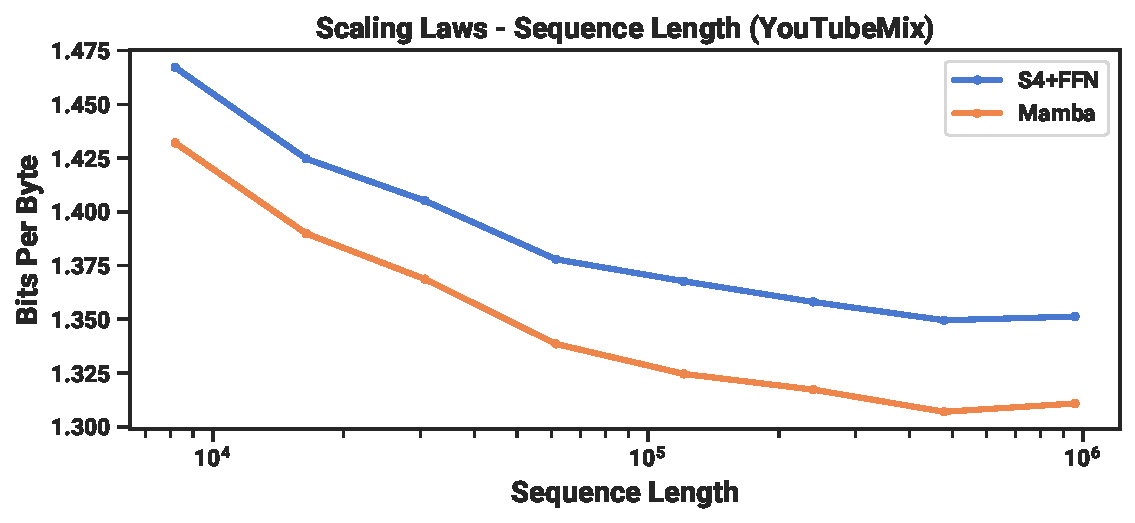
\includegraphics[width=\linewidth]{fig/youtubemix.pdf}
    \captionsetup{type=figure}
    \caption{
      (\textbf{Audio Pretraining}.) Mamba improves performance over prior state-of-the-art (Sashimi) in autoregressive audio modeling, while improving up to minute-long context or million-length sequences\iftoggle{arxiv}{ (controlling for computation)}{}.
    }
    \label{fig:youtubemix}
  \end{minipage}
\end{figure*}


\subsection{Audio Modeling and Generation}
\label{sec:exp:audio}

For the audio waveform modality, we compare primarily to the SaShiMi architecture and training protocols~\citep{goel2022raw}.
\iftoggle{arxiv}{
  This model comprises:
\begin{enumerate}
  \item a U-Net backbone with two stages of pooling by a factor $p$ that doubles the model dimension $D$ per stage,
  \item alternating S4 and MLP blocks in each stage.
\end{enumerate}
We consider replacing the S4+MLP blocks with Mamba blocks.
}{
  The architecture is a U-Net with alternating S4 and MLP blocks, which we consider replacing with Mamba.
}
  Experiment details are in \cref{sec:exp-details:audio}.

\iftoggle{arxiv}{
\subsubsection{Long-Context Autoregressive Pretraining}
}{
\para{Long-Context Autoregressive Pretraining.}%
}
We evaluate pretraining quality \iftoggle{arxiv}{(autoregressive next-sample prediction)}{} on YouTubeMix~\citep{deepsound},
a standard piano music dataset\iftoggle{arxiv}{ used by prior work consisting of $4$ hours of solo piano music, sampled at a rate of 16000 Hz}{}.
\iftoggle{arxiv}{Pretraining details largely follow the standard language modeling setup (\cref{sec:exp:language}).}{}
\cref{fig:youtubemix} evaluates the effect of increasing training sequence lengths from $2^{13}=8192$ to $2^{20}\approx 10^6$, while keeping computation fixed.
\iftoggle{arxiv}{
(There are some slight edge cases to the way the data is curated, which may lead to kinks in the scaling curves. For example, only minute-long clips were available so the maximum sequence length is actually bounded by $60s \cdot 16000Hz = 960000$.)

\textbf{Both Mamba and the SaShiMi (S4+MLP) baseline improve consistently with longer context lengths; Mamba is better throughout, and the gap widens at longer lengths.}
The main metric is bits per byte (BPB), which is a constant factor $\log(2)$ of the standard negative log-likelihood (NLL) loss for pretraining other modalities.

We note one important detail: this is the only experiment in this paper in which we switched from the real parameterization to complex (\cref{sec:method:details}).
We show additional ablations in \cref{sec:exp-details:audio}.
%
}{}


\iftoggle{arxiv}{
\subsubsection{Autoregressive Speech Generation}
}{
\para{Autoregressive Speech Generation.}
}
\iftoggle{arxiv}{
SC09 is a benchmark speech generation dataset~\citep{Warden2018SpeechCA,donahue2019adversarial}, consisting of $1$-second clips sampled at 16000 Hz of the digits ``zero'' through ``nine'' with highly variable characteristics. %
We largely follow the autoregressive training setup and generation protocol of \citet{goel2022raw}.

\cref{tab:sc09} shows automated metrics of the Mamba-UNet model compared to a variety of baselines from \citet{goel2022raw}:
WaveNet~\citep{oord2016wavenet}, SampleRNN~\citep{mehri2017samplernn}, WaveGAN~\citep{donahue2019adversarial}, DiffWave~\citep{kong2021diffwave}, and SaShiMi.
\textbf{A small Mamba model outperforms the state-of-the-art (and much larger) GAN- and diffusion- based models.}
A larger model parameter-matched to the baselines further improves on fidelity metrics dramatically.

\cref{tab:sc09-ablations} takes the small Mamba model and investigates combinations of different architectures for the outer stages and center stage.
It shows that Mamba is consistently better than S4+MLP in the outer blocks,
and Mamba $>$ S4+MLP $>$ MHA+MLP in the center blocks.
}{
  \cref{tab:sc09,tab:sc09-ablations} show results on the SC09 dataset for generating speech clips of the digits 0-9~\citep{Warden2018SpeechCA,donahue2019adversarial}.
  Mamba sets significant state-of-the-art results, and is consistently better than attention or S4 blocks in a parameter-controlled setting.
}

\begin{figure*}[!ht]
  \begin{minipage}[t]{.50\linewidth}
    \centering
    \captionsetup{type=table}
    \caption{
      (\textbf{SC09}) Automated metrics for unconditional generation on a challenging dataset of fixed-length speech clips.
      (\emph{Top to Bottom}) Autoregressive baselines, non-autoregressive baselines, Mamba, and dataset metrics.
    }
    \scriptsize
    \begin{tabular}{@{}lllllll@{}}
      \toprule
      \textsc{Model} & \textsc{Params} & \textsc{NLL $\downarrow$} & \textsc{FID $\downarrow$} & \textsc{IS $\uparrow$} & \textsc{mIS $\uparrow$} & \textsc{AM $\downarrow$}      \\
      \midrule
      SampleRNN      & 35.0M           & 2.042                     & 8.96                      & 1.71                   & 3.02                    & 1.76                                \\
      WaveNet        & 4.2M            & 1.925                     & 5.08                      & 2.27                   & 5.80                    & 1.47                                \\
      SaShiMi        & 5.8M            & 1.873                     & 1.99                      & 5.13                   & 42.57                   & 0.74                           \\
      \midrule
      WaveGAN        & 19.1M           & -                         & 2.03                      & 4.90                   & 36.10                   & 0.80                                \\
      DiffWave       & 24.1M           & -                         & 1.92                      & 5.26                   & 51.21                   & 0.68                                \\
      \;\; + SaShiMi & 23.0M           & -                         & 1.42                      & 5.94                   & 69.17                   & 0.59                           \\
      \midrule
      \textbf{Mamba} & 6.1M            & \textbf{1.852}            & \underline{0.94}          & \underline{6.26}       & \underline{88.54}       & \underline{0.52}                           \\
      \textbf{Mamba} & 24.3M           & \underline{1.860}         & \textbf{0.67}             & \textbf{7.33}          & \textbf{144.9}          & \textbf{0.36}                           \\
      \midrule
      Train          & -               & -                         & $0.00$                    & $8.56$                 & $292.5$                 & $0.16$                                \\
      Test           & -               & -                         & $0.02$                    & $8.33$                 & $257.6$                 & $0.19$                                \\
      \bottomrule
    \end{tabular}
    \label{tab:sc09}
  \end{minipage}
  \hfill
  \begin{minipage}[t]{.49\linewidth}
    \centering
    \captionsetup{type=table}
    \caption{
      (\textbf{SC09 Model Ablations}) Models with 6M parameters. In SaShiMi's U-Net backbone, there are 8 center blocks operating on sequence length $1000$, sandwiched on each side by 8 outer blocks on sequence length $4000$, sandwiched by 8 outer blocks on sequence length $16000$ (40 blocks total). The architecture of the 8 center blocks are ablated independently of the rest. Note that Transformers (MHA+MLP) were not tested in the more important outer blocks because of efficiency constraints.
    }
    \scriptsize
    \begin{tabular}{@{}lllllll@{}}
      \toprule
      \textsc{Outer} & \textsc{Center} & \textsc{NLL $\downarrow$} & \textsc{FID $\downarrow$} & \textsc{IS $\uparrow$} & \textsc{mIS $\uparrow$} & \textsc{AM $\downarrow$}      \\
      \midrule
      S4+MLP         & MHA+MLP         & 1.859                     & 1.45                      & 5.06                   & 47.03                   & 0.70 \\
      S4+MLP         & S4+MLP          & 1.867                     & 1.43                      & 5.42                   & 53.54                   & 0.65 \\
      S4+MLP         & Mamba           & 1.859                     & 1.42                      & 5.71                   & 56.51                   & 0.64 \\
      Mamba          & MHA+MLP         & \textbf{1.850}            & 1.37                      & 5.63                   & 58.23                   & 0.62 \\
      Mamba          & S4+MLP          & 1.853                     & \underline{1.07}          & \underline{6.05}       & \underline{73.34}       & \underline{0.55} \\
      Mamba          & Mamba           & \underline{1.852}         & \textbf{0.94}             & \textbf{6.26}          & \textbf{88.54}          & \textbf{0.52} \\
      \bottomrule
    \end{tabular}
    \label{tab:sc09-ablations}
  \end{minipage}
\end{figure*}


\iftoggle{arxiv}{
  \subsection{Speed and Memory Benchmarks}
\label{sec:exp:benchmark}


We benchmark the speed of the SSM scan operation (state expansion $N=16$), as well as the end-to-end
inference throughput of Mamba, in \cref{fig:scan_benchmark}.
Our efficient SSM scan is faster than the best attention implementation that we know of
(FlashAttention-2~\citep{dao2023flashattention2}) beyond sequence length 2K,
and up to 20-40$\times$ faster than a standard scan implementation in
PyTorch.
Mamba achieves 4-5$\times$ higher inference throughput than a Transformer of similar
size, since without the KV cache it can use much higher batch sizes.
For example, a Mamba-6.9B (untrained) would have higher inference throughput than a
$5\times$ smaller Transformer-1.3B.
Details in \cref{sec:exp-details:benchmark}, which additionally includes a benchmark of memory consumption.


}{}
\begin{figure*}[!th]
  \centering
  \begin{subfigure}{.5\textwidth}
    \centering
    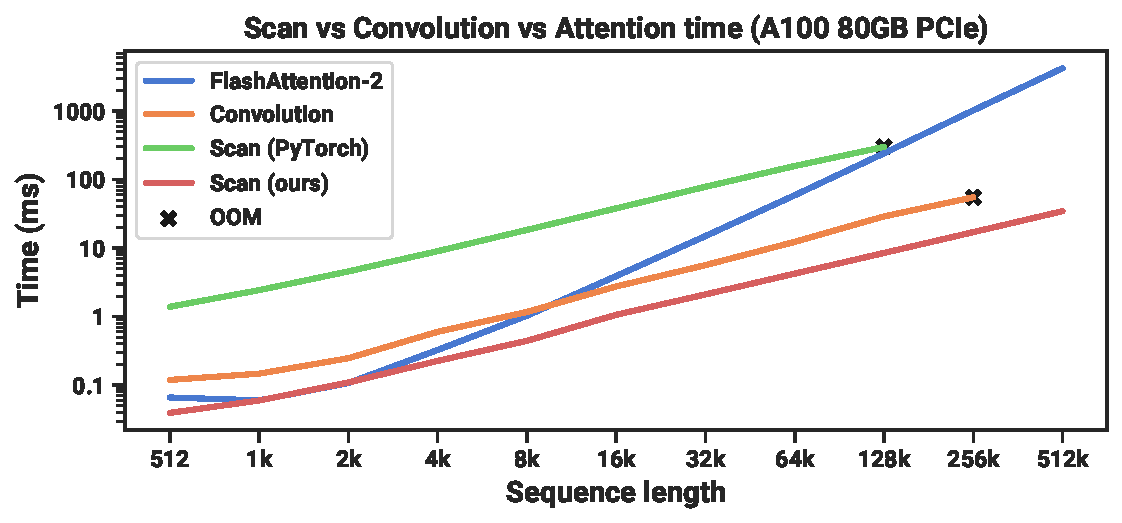
\includegraphics[width=.95\linewidth]{fig/ssm_scan.pdf}
  \end{subfigure}%
  \begin{subfigure}{.5\textwidth}
    \centering
    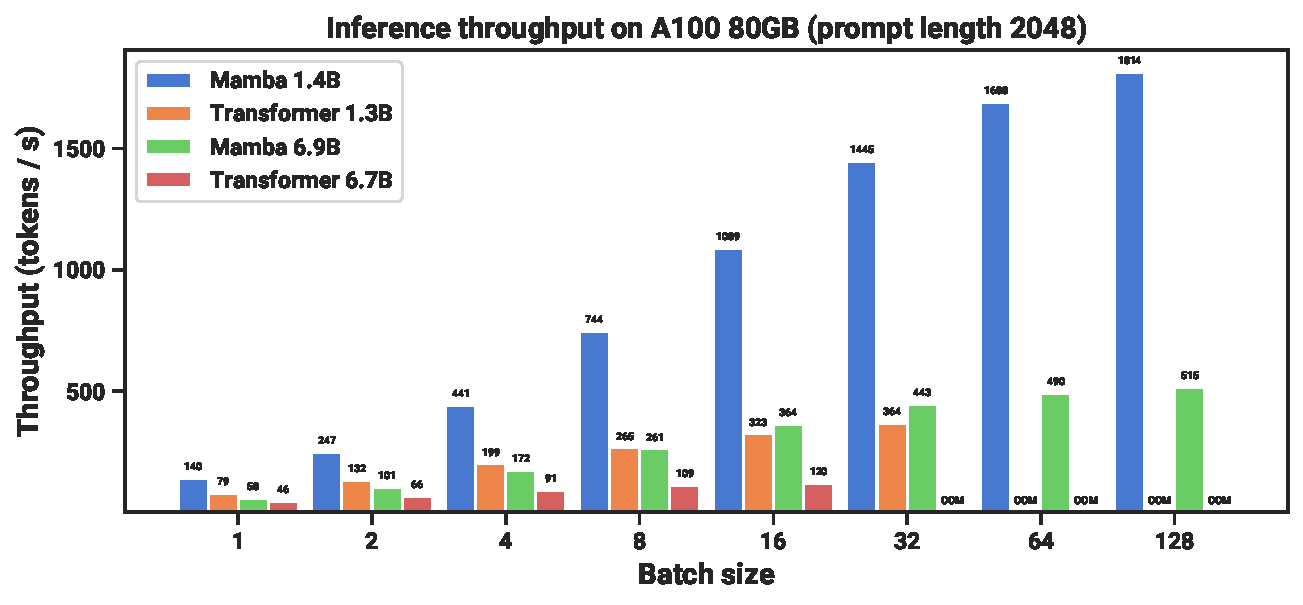
\includegraphics[width=.95\linewidth]{fig/mamba_inference.pdf}
  \end{subfigure}
  \caption{
    (\textbf{Efficiency Benchmarks}.)
    (\emph{Left}) Training: our efficient scan is $40\times$ faster than a standard implementation.
    (\emph{Right}) Inference: as a recurrent model, Mamba can achieve $5\times$ higher throughput than Transformers.
  }
  \label{fig:scan_benchmark}
\end{figure*}


\iftoggle{arxiv}{

  \begin{table}[h]
    % \captionsetup{font=small}
    \small
    \centering
    % \vspace{-1em}
    \caption{\label{table:ablations} Perplexity of SSM variants compared to
      Transformers on OpenWebText. All models have 12 layers, with size around 125M, and are trained
      with the same hyperpameters, for 50B tokens.}
    %   \vspace{1em}
    {
        \begin{tabular}{@{}|ccccc|c|@{}}
            \hline
        %   \specialrule{.15em}{.05em}{.05em}
        \hthree & \hthree Hybrid (2 Attn) & S4D & GSS & GSS Hybrid (2 Attn) & Transformer  \\ % & Training time \\
        %   \specialrule{.15em}{.05em}{.05em}
        \hline
        21.0 & \textbf{19.6} & 24.9 & 24.0 & 19.8 & 20.6 \\ \hline
        \end{tabular}
    }
    % \vspace{-1.5em}
\end{table}

}{
}


